%-----------------------------------------------------
% Chapter: Background 
%-----------------------------------------------------
\chapter{Background}
\label{chap:background}
This chapter provides an introduction to the theory and previous work within the areas of word embeddings, neural language models and text classification. 

\section{Word Embeddings}
Word embeddings are vectors of predefined size which aim to encode a distributional numerical representation of word features. They have found usage in a variety of applications such as document classification (REF) and named entity recognition (REF). Conceptually they exploit the idea that words which appear in a similar context have similar meanings. Recent aforementioned methods of learning these representations include both the GloVe and Word2Vec algorithms. Previous techniques for creating such representations can be categorised into two categories: matrix factorization methods and shallow window-based methods.
\subsection{Historic Methods}
\subsubsection{Global Matrix Factorization methods}
Global matrix factorization is the process of using matrix factorisation in order to perform rank reduction on a large term-frequency matrix. Within natural language processing, these matrices usually take one of two forms, term-document frequencies, where each entry represents the count of a particular word within a document, and term-term frequencies, which measures the co-occurrence of words within a given context. Matrix factorisation techniques such as Latent Sentiment Analysis (LSA) allow for fast training and perform well on word similarity tasks by leveraging word occurrence statistics however they suffer from the disproportionate importance given to large word counts.
\subsubsection{Shallow Window-Based methods}
Shallow window-based methods provide an alternative approach to learning word representations by sliding a fixed window over the contents of a corpus and learning to predict either the surroundings of a given word (skip-gram model) or predict a word given its surroundings (continuous bag of words). In the case of shallow window-based methods, they are good at capturing more complex patterns and do well in the word analogy task, however they fail to leverage global statistical information such as those used in global matrix factorization methods.
\subsection{GloVe - Global Vectors for Word Representation}
GloVe (Global vectors for word representation ) (REF) is an unsupervised word embedding algorithm, introduced by Pennington et al . (2014) which marries the benefits of both global matrix factorisation and shallow window based methods. Presented as a log-bilinear regression model, GloVe makes use of a global co-occurrence statistics from a corpus. As detailed in the paper, Glove outperformed previous methods such as Word2vec in word analogy, word similarity and named entity recognition tasks. Conceptually, GloVe is based on the idea that ratios of probabilities of words co-occurring have the potential to encode meaning which is encoded as vector differences. This concept is formalised in the following equation, where the dot product of focal and context word vectors, \(w\) and \(\tilde{w}\), is equal to the logarithm of the probability of the words co-occurring, \(\log{X_{ij}}\).

\begin{equation}
w_{i}^{T} \tilde{w_{j}} + b_{i} + \tilde{b}_{j} = \log{X_{ij}}^{2}
\end{equation}

\noindent
\newline
A weighting function \(f(X_{ij})\) is used to decrease noise caused by very frequent word co-occurrences. The following weighting function is used in the GloVe model.

\begin{equation}
	f(x) =
	\begin{cases}
	(x/x_{max}), & \text{if  \(x <\) } x_{max} \\
	1, & \text{otherwise}
	\end{cases}
\end{equation}

\noindent
\newline
Combining equations 3.1 and 3.2, the GloVe model is defined as a weighted least squares regression problem.
\begin{equation}
	J = \sum_{i, j=1}^{N} f(X_{ij}) (w_{i}^{T} \tilde{w_{j}} + b_{i} + \tilde{b}_{j} - \log{X_{ij}})^{2}
\end{equation}
\subsection{CoVeR - Covariate-Specific Word Embeddings}
Covariates such as author demographics, time and location often accompany documents within a corpus. A trivial approach to learning covariate specific word embeddings would involve applying GloVe to each subset of a corpus relating to a particular covariate. A weakness in this approach is that information from each of the specific covariate co-occurrence matrices is not shared.

\noindent
\newline
CoVer, proposed by Tian et al Stanford, provides an alternative to the conditional GloVe method. Being an extension of GloVe, CoVer extends Glove's matrix decomposition of co-occurrence matrices to tensor decomposition of co-occurrence tensors, involving the joint learning of word embeddings and covariate specific transformation matrices which represent the effect of a particular covariate on the base embeddings learned. The CoVeR model is presented below.

\begin{equation}
J = \sum_{i, j=1}^{N} \sum_{k=1}^{M} f(X_{ijk}) ((c_{k} \odot w_{i})^{T} (c_{k} \odot \tilde{w}) + b_{ik} + \tilde{b}_{jk} - \log{X_{ijk}})^{2}
\end{equation}


\section{Language Models}
Formal languages such as programming languages are fully specified with precise syntax and semantics which dictate the usage of all reserved words within a language. Contrarily, natural languages, because of their emerging nature, are unable to be formally specified even with the existence of grammatical rules and structures. Unfortunately, rule based systems suffer from the endless possibilities of language usage outside of grammatical rules which are still easily interpretable by humans. Moreover the task of consistently updating rule based systems to accommodate such usage is suboptimal.  

\noindent
\newline
Language modelling is the task of estimating the probability distribution of various linguistic units such as characters, words and sentences. In recent years, the application of LM  has been essential to many natural language process tasks such as speech to text and text summarization. Language models can be classified into two categories, count-based and continuous-space language models. 

\subsection{Count Based Models}
Count based methods such as statistical language models attempt to create the joint probability distribution of a sequence of words. An example of a count based method is the n-gram model.

\noindent
\newline
An n-gram is a sequence of N words. Examples of a two word sequences or bigrams include, "My name" and "is Aubrey", whilst examples of three word sequences or trigrams, include sequences such as "Hello my name" and "is Aubrey Graham". The n-gram model which considers the past n-1 words can be formailsed as 

\noindent
\newline
The n-gram model relies on Markov assumptions to model the probability of word sequences P(w1....wm) as being equal to a limited number of previous words. An inherent problem with the n-gram model is sparsity as some word sequences occur rarely or not at all, even in large text corpora. Using the standard n-gram model would yield to many zero probabilities. To circumvent this, techniques such as back-off and smoothing exist. Another disadvantage of n-gram models is that they rely on exact patterns, meaning n-gram models fail to recognise syntactically and semantically similar sentences such as "the cat sat on the mat" and "the dog sat on the mat". N-gram models also suffer from the curse of dimensionality due to increased vocabulary sizes. As a result, limited window sizes are used, causing longer dependencies between words to not be captured.

\noindent
\newline
To overcome these issues, deep learning methods have been used to create neural language models by simultaneously learning word embeddings and the parameters needed to create a joint probability distribution between the word embeddings. Bengio et al (2003) proposed a feed forward neural language model to help tackle the problem of data sparsity. Recent state of the art approaches have implored recurrent neural networks to help longer dependencies between sequences.
 

\subsection{Neural Language Models}
\subsubsection{Artificial Neural Networks}
In any neural network architecture, the elementary unit of computation is the artificial neuron which takes inspiration from biological neurons. The artificial neuron receives \(n\) inputs which are each weighted by \(n\) weights and summed together with a bias \(b\). The output \(y\) of a neuron is calculated by passing the weighted sum of the inputs into an activation function \(f\). 

\begin{equation}
	y = \sum_{i=1}^{N} x_{i}w_{i} + b
\end{equation}

\noindent
\newline
Typical activation functions include \textit{Sigmoid}, \textit{Tanh} and \textit{ReLu}. A single layer neural network is defined by \(k\) neurons sharing the same input in the same layer. Single layer neural networks have been proven to be \textit{'universal approximators'} meaning any continuous function can be approximated using this type of network. The process of stacking layers on top of each other leads to multi-layer neural networks. These types of networks are also known as feed-forward networks. The learnable parameters of these networks are the set of weights and biases for each layer. A feed-forward neural network is trained using gradient descent and its parameters are updated using the \textit{backpropagation} algorithm (REF).

\begin{figure}[h]
	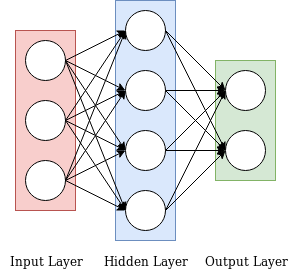
\includegraphics[width=8cm, height=8cm]{./figures/fig2}
	\centering
	\caption{Example neural network, three input nodes, four hidden and two outputs}
	\label{fig:fig2}
\end{figure}

\subsubsection{Recurrent Neural Network}
In a feed-forward neural network, data flow is unidirectional between layers; with data passing through a given neuron at most once. These types of networks perform well on both classification and regression tasks with the assumption that inputs are independent of each other. In tasks dealing with sequential data, feed-forward networks perform poorly. To model sequential data well, a neural network must be able to model the dependencies that exist between successive inputs. The recurrent neural network (RNN) is an attempt to satisfy this requirement by utilising past inputs to help predict future outputs.
\par
\noindent
\newline
In an RNN information is cycled within the network at least once.  An RNN receives a sequence of inputs \(x\) and updates its hidden state \(h_{t}\) by 

\begin{equation}
	h_{t}=
	\begin{cases}
	 0, & \text{t = 0} \\
	 \phi{(h_{t-1}, x_{t})}, & \text{otherwise}
	\end{cases}
\end{equation}

\noindent
where $\phi$ is a nonlinear function such as \textit{tanh} or \textit{ReLu}. The update for the hidden state is usually implemented as 

\begin{equation}
h_{t} = \phi{(Ux_{t} + Wh_{t-1})}
\end{equation}

\noindent
where W and U are weight matrices.

\par
\noindent
\newline
RNN's are trained using gradient descent and backpropagation through time (BBTT), which is identical to performing backpropagation on an \textit{"unrolled"} RNN; DESCRIBE UNROLLED RNN.

\begin{figure}[h]
	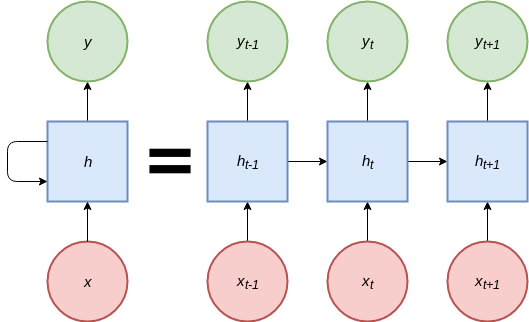
\includegraphics[width=10cm, height=6cm]{./figures/fig3}
	\centering
	\caption{\textit{Unrolled} Recurrent Neural Network}
	\label{fig:fig3}
\end{figure}

\par
\noindent
\newline
In BBTT, the gradient is back-propagated through network layers at each time step to adjust weights accordingly. During this process, weights in each layer are adjusted using previous gradients from output layers causing gradients to become increasing smaller. Ever decreasing gradients, or "vanishing gradients", can prevent the network from learning entirely due to the minimal updates applied to weights in earlier layers.

\subsubsection{Long Short-Term Memory}
Long Short-Term Memory (LSTM) (Hochreiter, 1997) is a variant of the recurrent neural network which is capable of capturing longer dependencies between sequences of data without suffering from vanishing gradients. This is achieved through a feature known as gating; a mechanism which acts as a permissive or restrictive barrier to information flow. 

\noindent
\newline
The core component of the LSTM is the cell state which is able to propagate \textbf{relevant} information throughout the network. This is achieved within the memory cell through the forget, input and output gate. The forget gate regulates how much of the existing memory should be forgotten, the input gate regulates how much of the new cell state to keep, and the output gate regulates how much of the cell state should be allowed into the next layer of the network.

\begin{figure}[h]
	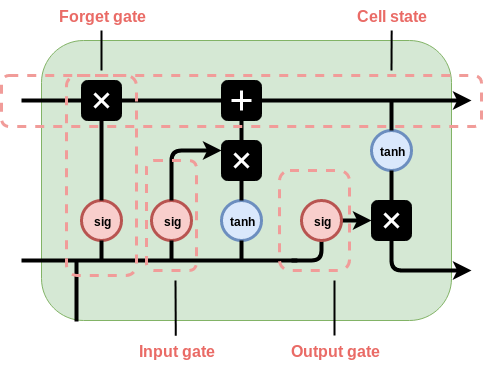
\includegraphics[width=10cm, height=8cm]{./figures/fig4}
	\centering
	\caption{LSTM memory cell, with forget, input and output gates}
	\label{fig:fig3}
\end{figure}

\subsubsection{Neural Language Models}
RNN's have been used successfully in a range of NLP tasks such as language modelling (Bengio et al. (2006)) and statistical machine translation (Cho et al. (2014)) Mikolov et el, abstracts statistical language models as a form of sequential data prediction. Unlike Bengio et al, feed-forward neural network architecture, the paper takes advantage of the recurrent connections within an RNN. 

\subsection{Text Classification}
Text classification is the task of assigning pre-defined labels to text according to its content. Automated classification of text can be achieved through rule based and machine learning based systems. Rule based methods tackle classification through the use of handcrafted linguistic rules, which assign patterns in text to predefined categories. For example, given two word lists which  Rule based systems don't come without drawbacks, firstly to create such a system requires deep domain knowledge. Moreover, unlike the previous example, creating, maintaining and scaling such rules is challenging and time consuming. 
\subsubsection{Traditional Methods}
\paragraph{Naive Bayes} 
Naive Bayes Classification is a generative approach which uses bayes theorom to learn a join probability distribution .... Naive bayes classification is a robust method for training a text classifier which can achieve accurate results without large amounts of training data.

Naive bayes is a classification techinque based on bayes theroem with an assumpoion of inde[endence among preictors. A naives bayes c;assifier assumes that the precence of a particular fgeature in a class is unrelsted tp the [recence of any other fetaure.

\paragraph{Support Vector Machines}
A Support Vector Machines (SVM) (Vapnik et al 1995) is a discriminative classifier that aims to find a linear classification boundary or \textit{hyperplane} to discriminate between classes in high dimensional space. SVM's achieve this through support vectors, random training data points, which are used to maximise the margin between ... Similar to naive bayes classifiers, SVM's do not require large amounts of training data to achieve accurate results. SVM's were introduced to the problem of text classification by Joachims(REF)

\subsubsection{Deep Learning Methods}